\section{Transformers}

\subsection{Some limitations of our approaches so far}

\begin{frame}{Some problems to address}
  Just replacing BOW with word embeddings is not enough:
  \begin{block}{Context}
      \begin{itemize}
      \item ``bank'' (money), ``bank'' (of a river), \ldots $\rightarrow$ all the same word embedding
      \item Understanding references within a sentence (`` who is `she'?'') $\rightarrow$ can actually be done with, for instance, LSTM/RNN
      \end{itemize}
  \end{block}
\end{frame}

\begin{frame}{Some problems to address}
  
  \begin{block}{Tha amount of training data}
      \begin{itemize}
      \item Thousands of annotations needed in traditional BOW
      \item Especially be problematic when we have many and/or small categories
      \item We already argued that pre-trained embeddings can partly mitigate this
      \item Yet, a human doesn't need hundreds of examples but just a few to learn the difference between, say, two animal species (few-shot learning)
      \end{itemize}
  \end{block}
\end{frame}


\begin{frame}{``Attention  is all you need''}
  \begin{itemize}
  \item Title of an extremely influential paper \parencite{Vaswani2017}
  \item Paradigm shift:
  \end{itemize}

 \pause
 \begin{quote}
``The dominant sequence transduction models are based on complex recurrent or
convolutional neural networks that include an encoder and a decoder. The best
performing models also connect the encoder and decoder through an attention
mechanism. We propose a new simple network architecture, the Transformer,
based solely on attention mechanisms, dispensing with recurrence and convolutions
entirely.''
\end{quote}
\end{frame}

\begin{frame}[plain]
  OK, that sounds complicated.
\end{frame}

\begin{frame}{``Attention  is all you need''}
\begin{figure}
	\centering
	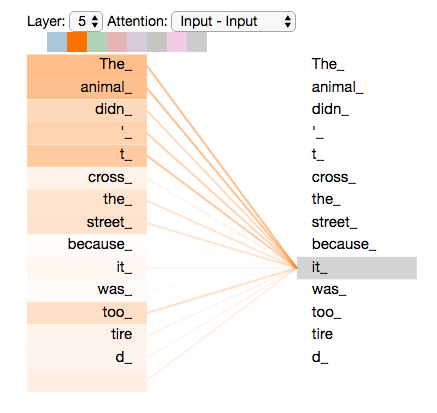
\includegraphics[width=.5\linewidth]{transformer_self-attention_visualization.png}
	\caption{The idea of ``attention''. \url{http://jalammar.github.io/illustrated-transformer/}}
	\label{fig:attention}
\end{figure}
\end{frame}


\begin{frame}{The technical details}
  We will not go into all the math behind it -- it's beyond the scope of this class. But there is a nice hands-on explanation of the \textcite{Vaswani2017}-paper including a commented Python implementation available at  \url{http://nlp.seas.harvard.edu/annotated-transformer/}.

  (Further reading if you consider to continue working on this)
\end{frame}


\subsection{BERT, the game changer}

\begin{frame}{Bidirectional Encoder Representations from Transformers}
The famous BERT \parencite{Devlin2018} model

\begin{quote}
`` The
masked language model randomly masks some of
the tokens from the input, and the objective is to
predict the original vocabulary id of the masked word based only on its context. Unlike left-to-
right language model pre-training, the MLM ob-
jective enables the representation to fuse the left
and the right context, which allows us to pre-
train a deep bidirectional Transformer. In addi-
tion to the masked language model, we also use
a “next sentence prediction” task that jointly pre-
trains text-pair representations.''
    \end{quote}

\end{frame}





\begin{frame}{The idea of finetuning}
  \begin{itemize}
  \item BERT (or GPT-4, \ldots) are Large Language Models (LLMs)
  \item Training them is \emph{really} expensive. Training BERT is said to have cost 7,000 USD, GPT-3 even 4,600,000 USD (just for the computing!) 
  \item So, no, you don't do that yourself (nor do universities, normally).
  \item Solution: Separating (unsupervised) pre-training from fine-tuning for downstream tasks!
  \end{itemize}

\end{frame}


\begin{frame}{Pre-training vs fine-tuning}
\begin{figure}
	\centering
	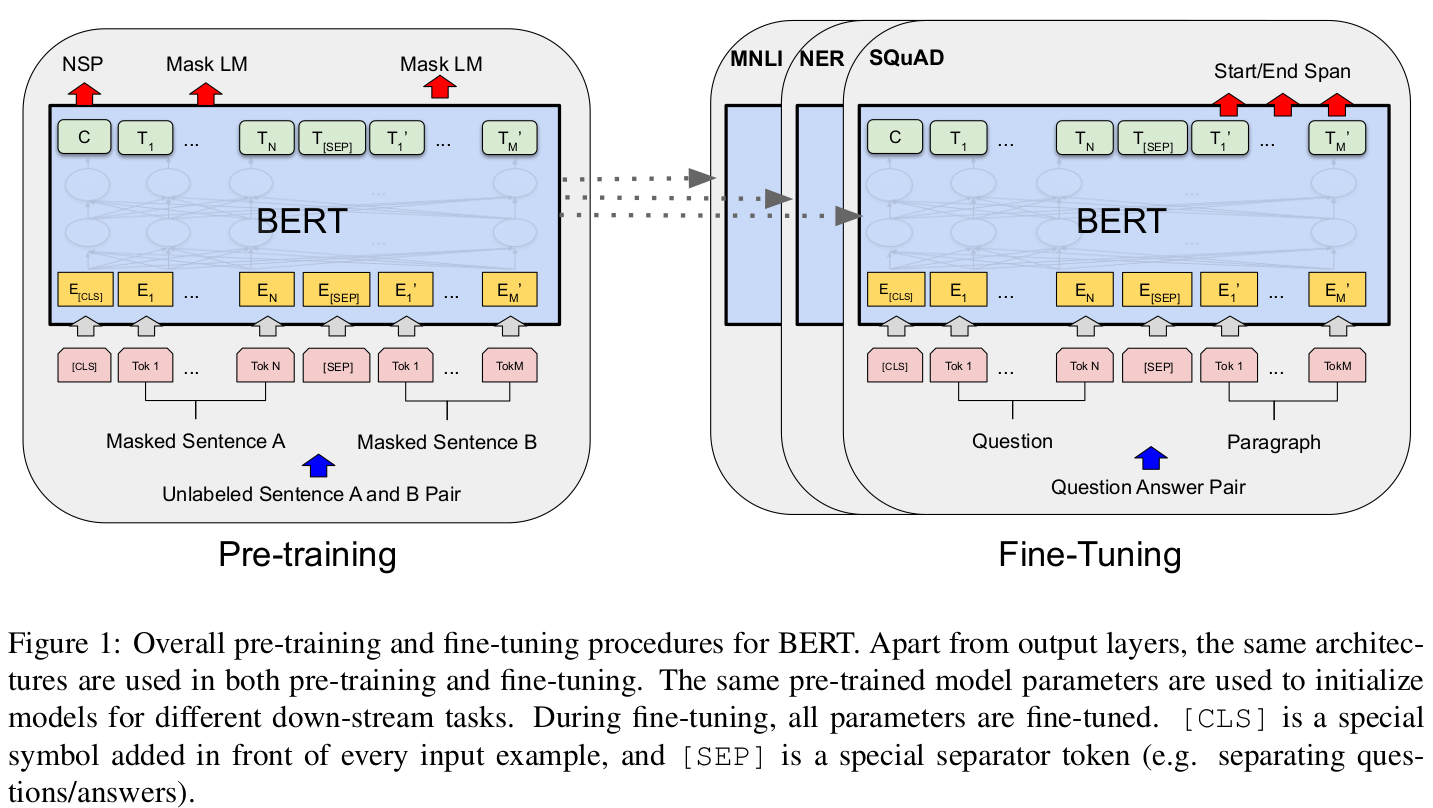
\includegraphics[width=.8\linewidth]{BERT-finetuning.png}
	\caption{Finetuning BERT \parencite{Devlin2018}.}
	\label{fig:finetuning}
\end{figure}

\end{frame}


\begin{frame}{How to fine-tune}
General idea: you download a pre-trained model, than finetune it 
  
  \begin{itemize}
  \item \url{https://www.huggingface.co} is your starting point
  \item We also made an example notebook: \url{https://github.com/uvacw/teaching-bdaca/blob/main/modules/machinelearning-text-exercises/transformers_bert_classification.ipynb}
  \item You probably want to use a GPU (e.g., on Google Colab)
  \end{itemize}

\end{frame}


\begin{frame}{How to fine-tune}
Note that you can fine-tune for very differnet tasks:
  
  \begin{itemize}
  \item classification ($\rightarrow$ SML)
  \item question answering
  \item translation
  \end{itemize}
\end{frame}


\question{Do you see how this relates to public-facing applications like DALL-E and ChatGPT? Do you see how these relate to encoding, decoding, and transformers?}




\subsection{Critical voices}


\begin{frame}{Stochastic parrots?}
Really read the paper by \parencite{Bender2021}!

Think about:

\begin{itemize}
\item environmental and financial costs
\item bias
\item ethical issues
\item ``amplification of a hegemonic worldview''
\item \ldots
\end{itemize}
  
\end{frame}








\subsection{Practical example}


\begin{frame}{\textcite{Lin2023}}

  Can we train a model to rate news items \emph{from very different sources such as newspaper articles, videos, podcasts, blogs, \ldots } on two scales
  \begin{enumerate}
  \item informal --- formal
  \item factual --- opinionated
  \end{enumerate}
to identify/describe their genre?
\end{frame}


\begin{frame}[plain]
\begin{figure}
	\centering
	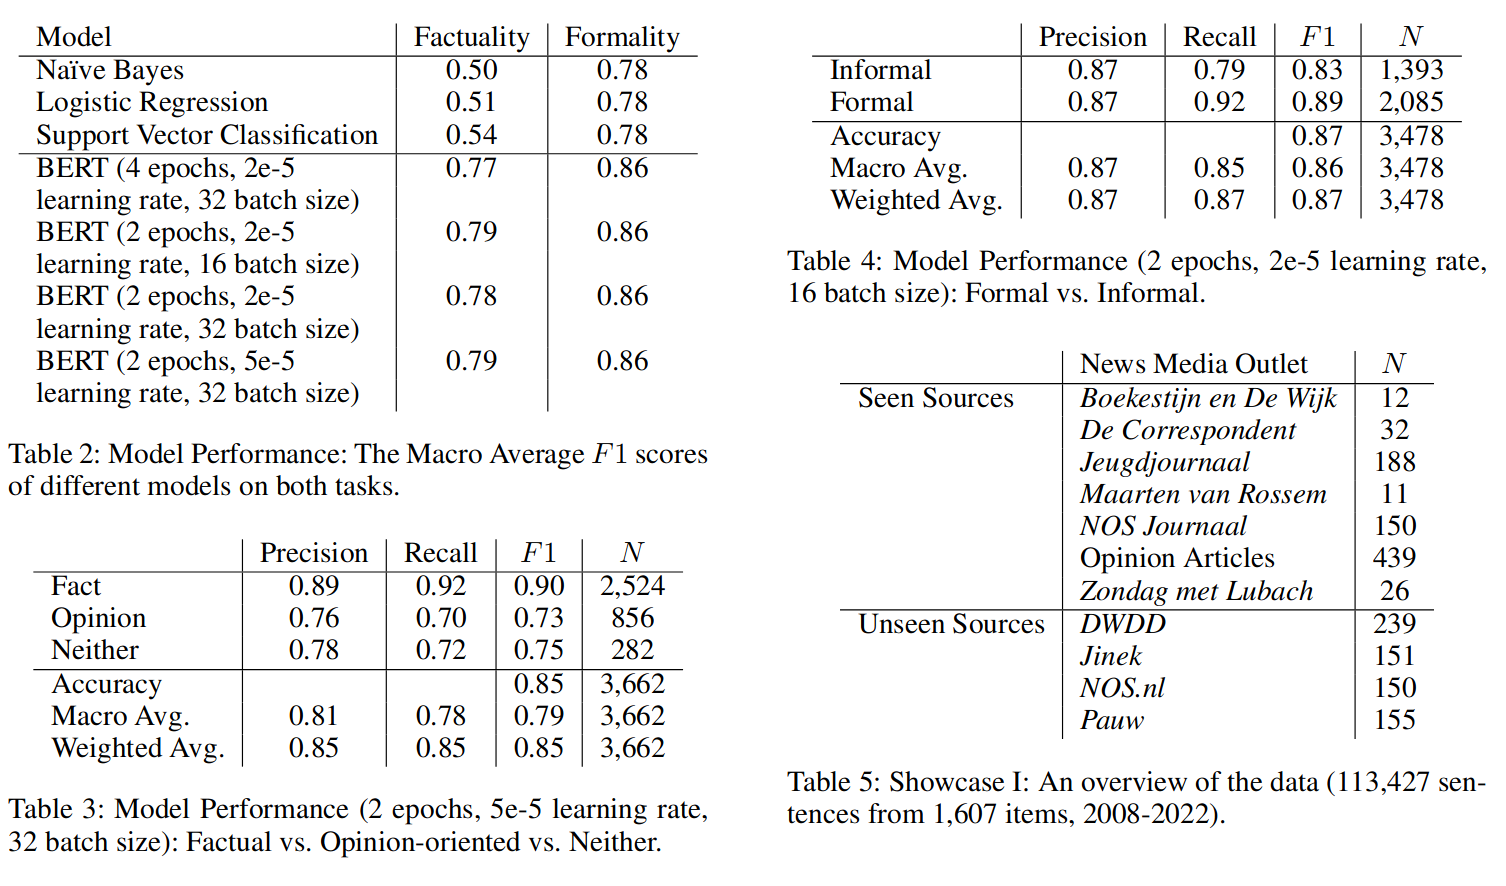
\includegraphics[width=\linewidth]{lin2013-1.png}
\end{figure}
\end{frame}


\begin{frame}[plain]
\begin{figure}
	\centering
	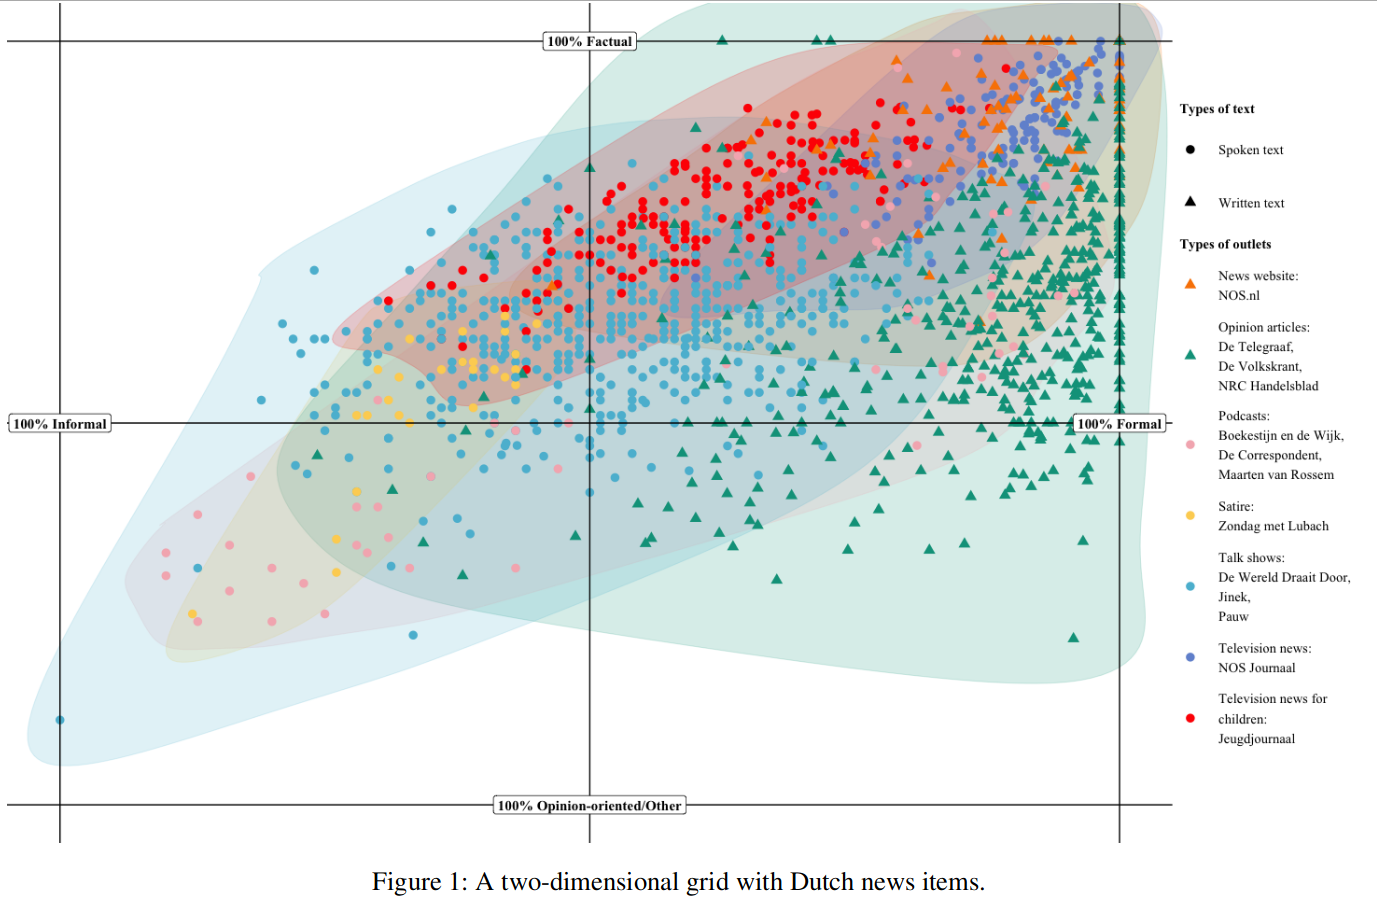
\includegraphics[width=\linewidth]{lin2013-2.png}
\end{figure}
\end{frame}


\begin{frame}[plain]
\begin{figure}
	\centering
	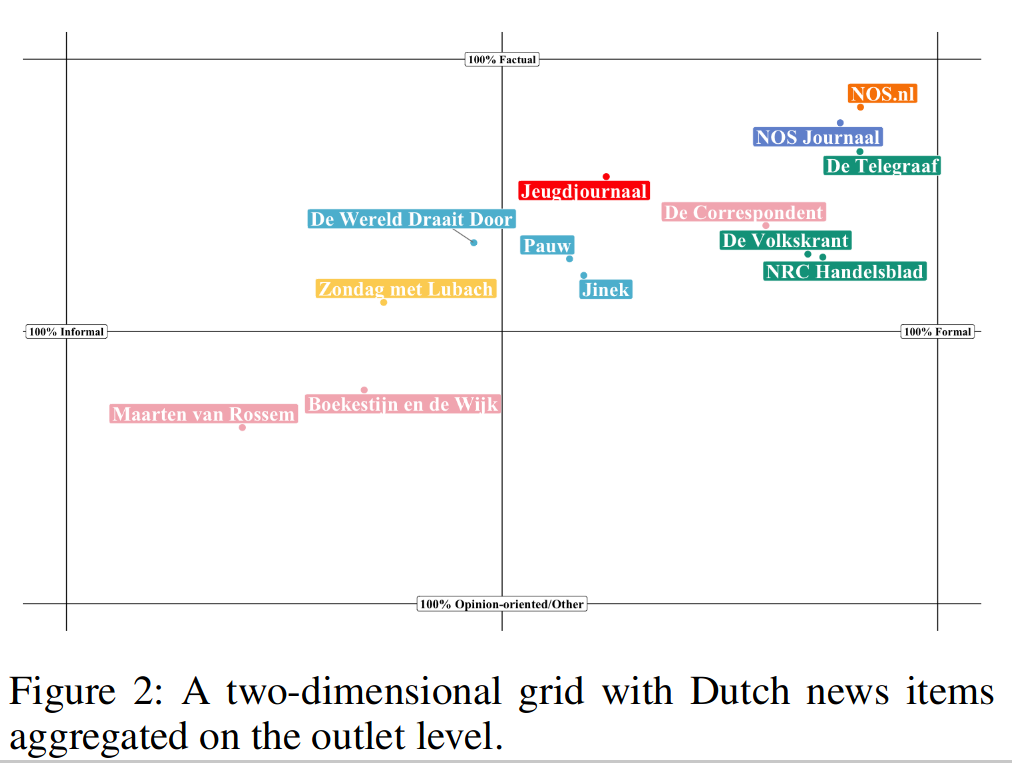
\includegraphics[width=\linewidth]{lin2013-3.png}
\end{figure}
\end{frame}


\begin{frame}{\textcite{Lin2023}}
  \begin{itemize}
  \item BOW approaches cannot achieve this well enough, but finetuning a transformer can
  \item They can generalize across \emph{very} different formats
  \end{itemize}

\end{frame}





\begin{frame}{Finally: Some links}
\begin{itemize}
\item \url{https://nlp.seas.harvard.edu/2018/04/03/attention.html}
\item \url{http://jalammar.github.io/illustrated-transformer/}
\end{itemize}
\end{frame}



